\chapter{Data matters}
\label{chp3}

\section{Feeling the heat}

Nel Capitolo \ref{chp2} si sono presentati i canali attraverso i quali il cambiamento climatico genera inflazione e influenza la politica monetaria.

In questo terzo e ultimo Capitolo si approfondirà empiricamente il ruolo della temperatura, quindi del riscaldamento globale, quale determinante delle variazioni dei prezzi. La trattazione si baserà sul recente \textit{Working Paper ECB "Feeling the heat: extreme temperatures and price stability"} pubblicato nel dicembre 2021 da Donata Faccia e altri \parencite{ECB:feeling_heat}.

\begin{figure}[h]
	\centering
	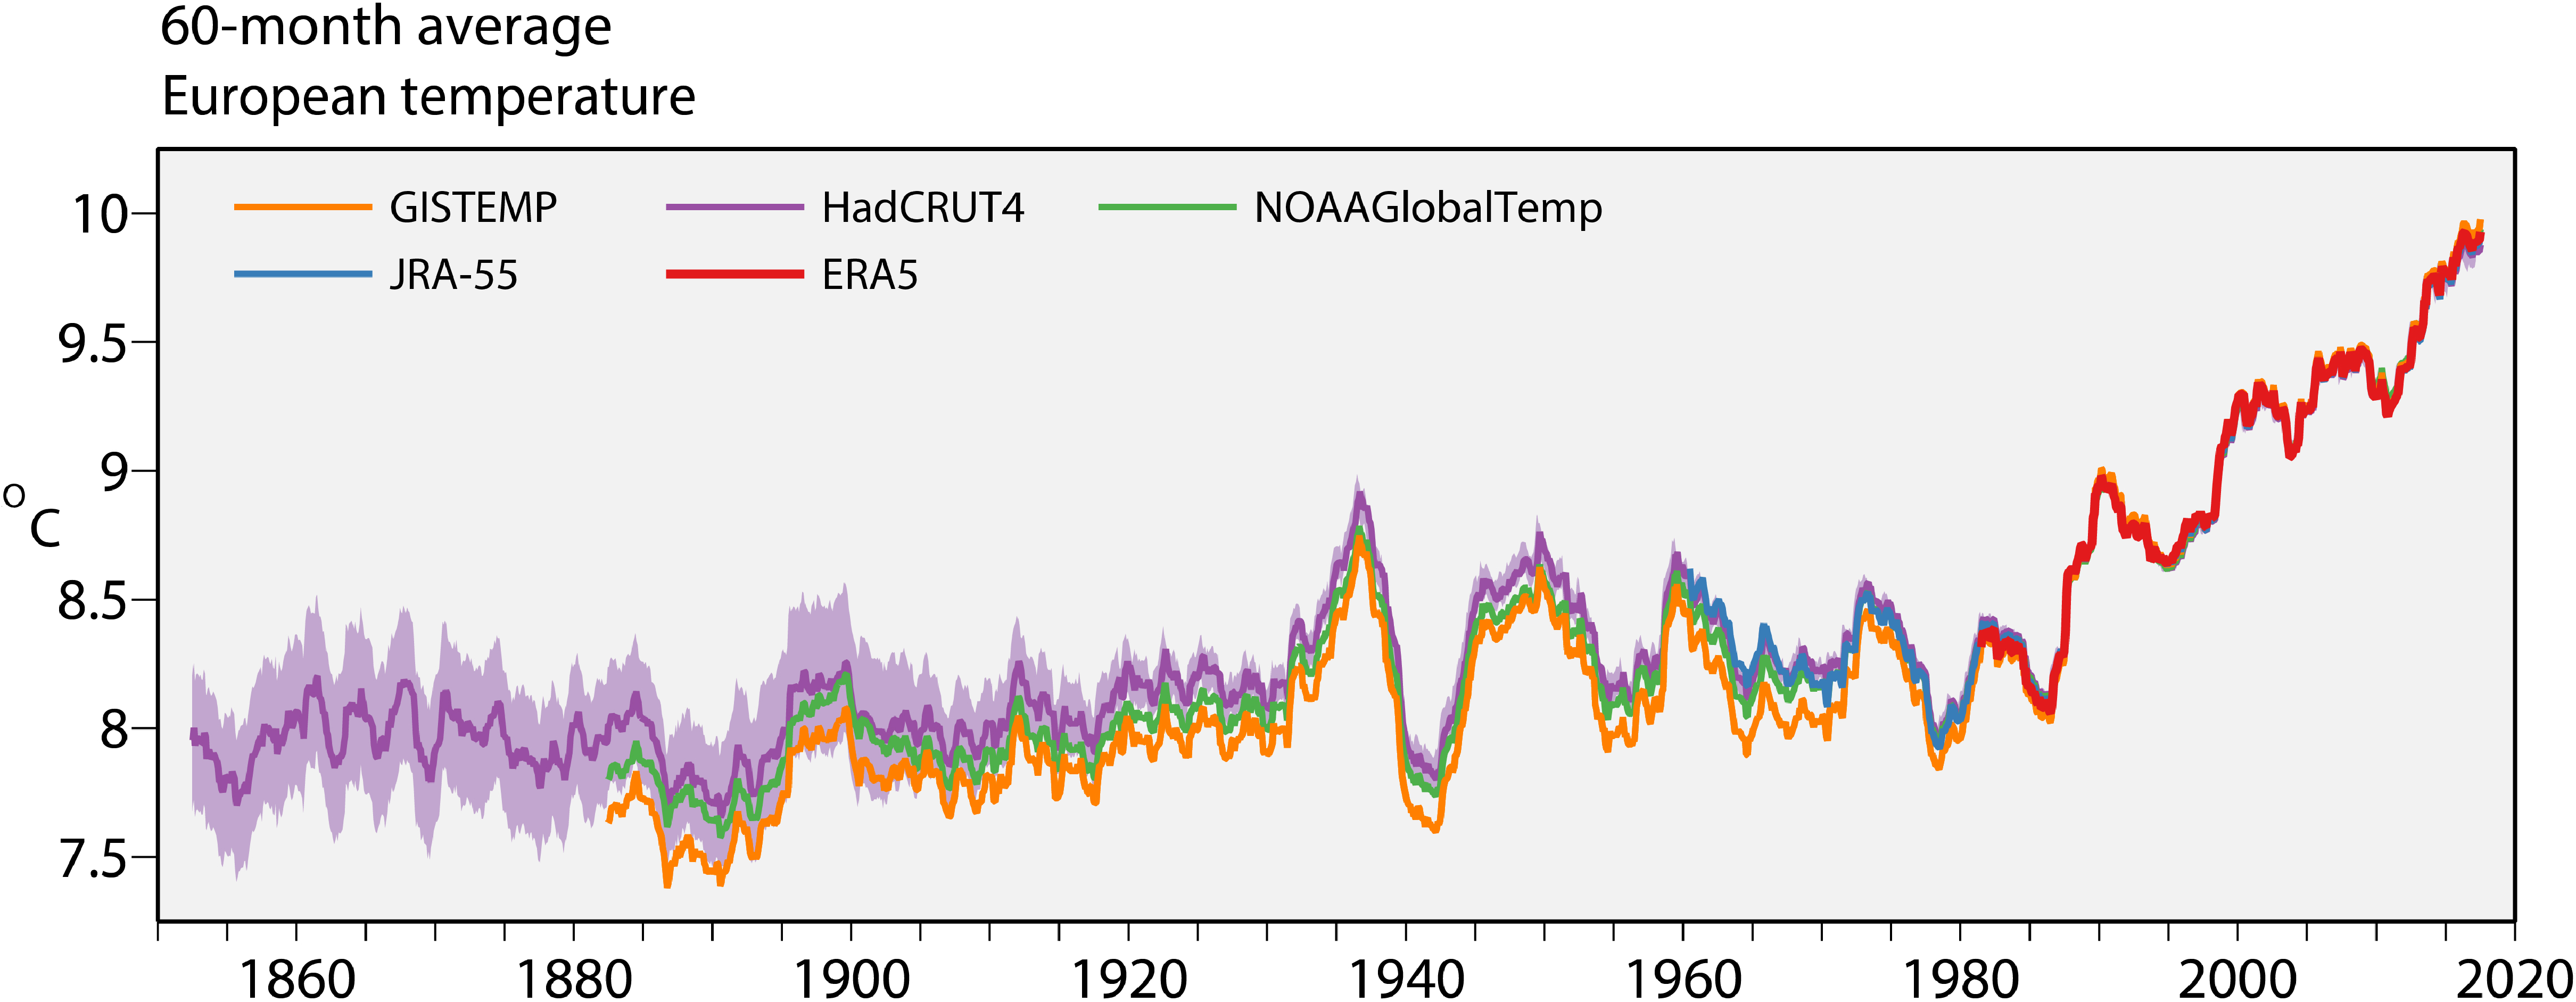
\includegraphics[width=0.80\textwidth]{img/europe_temp.pdf}
	\caption{}
	\source{\cite{Cop:global_temp}}
	\label{img:europe_temp}
\end{figure}

\noindent\begin{minipage}{\textwidth}
Come mostrato in Figura \ref{img:europe_temp}, il 2020 è stato l'anno più caldo in assoluto per l'Europa e, a queste condizioni, le temperature dei prossimi anni non accennano a diminuire. Nel Capitolo \ref{chp1} si è brevemente illustrato come la nostra atmosfera stia sempre più accumulando calore, con la principale conseguenza che gli eventi atmosferici estremi stanno diventando sempre più frequenti. La letteratura che studia questi fenomeni è ricca di pubblicazioni e, a supporto della trattazione successiva, se ne riportano alcune.
\end{minipage}

\textit{"Temperature Shocks and Economic Growth: Evidence from the Last Half Century"} pubblicato nel luglio 2012 da Melissa Dell e altri \parencite{Dell:temperature}. Confronta temperature e precipitazioni con la produzione aggregata del periodo 1950-2003. Conclude che in presenza di temperature maggiori, i livelli di output e i tassi di crescita si riducono. Inoltre, le crescenti temperature minano la produzione agricola, industriale e la stabilità politica.

\textit{"Temperature and Growth: A Panel Analysis of the United States"} pubblicato nel marzo 2019 da Riccardo Colacito e altri \parencite{Colacito:temp}. Analizza le temperature e l'output degli Stati Uniti d'America tra il 1957 e il 2012. Utilizza dati con frequenza trimestrale e ciò permette di studiare l'impatto degli aumenti di temperatura nelle diverse stagioni. In estate, l'aumento di un 1°F riduce la produzione aggregata di circa 0.15-0.25\%. Al contrario, autunni più miti, hanno effetti positivi sul PIL. Una possibile spiegazione fornita dagli autori è che durante le estati particolarmente calde la produttività del lavoro si riduce.

\subsection{I dati utilizzati}


\begin{table}[h]
	\centering
	\begin{tabularx}{.8\textwidth}{XXX}
		\toprule
		\multicolumn{2}{l}{\textbf{Advanced economies}} &
		\multicolumn{1}{l}{\textbf{Emerging economies}} \\ \midrule
		\begin{tabular}[t]{@{}l@{}}Austria\\ Australia\\ Belgium\\ Cyprus\\ Czechia\\ Denmark\\ Estonia\\ Iceland\\ Finland\\ France\\ Germany\\ Greece\\ Ireland\\ Israel\\ Italy\\ Japan\\ Korea\end{tabular} &
		\begin{tabular}[t]{@{}l@{}}Latvia\\ Lithuania\\ Luxembourg\\ Malta\\ Netherlands\\ New Zealand\\ Norway\\ Portugal\\ Singapore\\ Slovakia\\ Slovenia\\ Spain\\ Sweden\\ Switzerland\\ United Kingdom\\ United States\end{tabular} &
		\begin{tabular}[t]{@{}l@{}}Bulgaria\\ Brazil\\ Chile\\ China\\ Costa Rica\\ Croatia\\ Hungary\\ Malaysia\\ Mexico\\ Paraguary\\ Peru\\ Philippines\\ Poland\\ Thailand\\ Turkey\end{tabular}
		\\ \bottomrule
	\end{tabularx}
	\caption{}
	\source{\cite{ECB:feeling_heat}}
	\label{elenco_completo}
\end{table}

La recente pubblicazione di Donata Faccia studia l'impatto che gli shock di temperatura hanno sui prezzi di un paese. L'analisi si concentra sui dati aggregati di 48 paesi, l'elenco completo è in Tabella \ref{elenco_completo}, di cui 33 classificati come avanzati e 15 come emergenti.

La serie storica si sviluppa tra il 1990 e il 2018. La frequenza dei dati è trimestrale perché, come suggerito anche dallo studio di Riccardo Colacito \parencite{Colacito:temp}, questo permette di far emergere eventuali differenze che intercorrono nelle diverse stagioni.

Per garantire la massima completezza informativa, i dati dei prezzi provengono da diversi dataset e riguardano cinque diversi indici di prezzo: prezzi al consumo di tutti i beni (headline CPI), prezzi al consumo cibo (Food), prezzi al consumo non cibo (Non-Food), prezzi alla produzione e deflatore del PIL.

\begin{table}[h]
	\centering
	\begin{tabularx}{.8\textwidth}{@{}XXXXXX@{}}
		\toprule
		\textbf{Period} & \textbf{p10} & \textbf{p25} & \textbf{Median} & \textbf{p75} & \textbf{p90} \\ \midrule
		\textbf{Summer} &              &              &                 &              &              \\
		1990s           & -0.11        & 0.22         & 0.57            & 1.04         & 1.65         \\
		2000s           & 0.24         & 0.54         & 0.92            & 1.42         & 1.96         \\
		2010s           & 0.43         & 0.83         & 1.26            & 1.80         & 2.44         \\
		\textbf{Autumn} &              &              &                 &              &              \\
		1990s           & -0.69        & -0.15        & 0.31            & 0.76         & 1.17         \\
		2000s           & -0.11        & 0.33         & 0.71            & 1.08         & 1.71         \\
		2010s           & 0.16         & 0.63         & 1.02            & 1.46         & 2.01         \\
		\textbf{Winter} &              &              &                 &              &              \\
		1990s           & -0.70        & 0.07         & 0.74            & 1.49         & 2.61         \\
		2000s           & -0.55        & 0.13         & 0.80            & 1.65         & 2.69         \\
		2010s           & -0.57        & 0.21         & 0.90            & 1.69         & 2.99         \\
		\textbf{Spring} &              &              &                 &              &              \\
		1990s           & -0.25        & 0.20         & 0.66            & 1.21         & 1.72         \\
		2000s           & 0.16         & 0.54         & 1.00            & 1.68         & 2.31         \\
		2010s           & 0.24         & 0.69         & 1.37            & 2.03         & 2.57         \\ \bottomrule
	\end{tabularx}
	\caption{}
	\source{\cite{ECB:feeling_heat}}
	\label{table:distribuzione_anomalie}
\end{table}

\noindent\begin{minipage}{\textwidth}
A quelli sui prezzi si uniscono i dati sulle temperature. In particolare, ciò su cui ci si interroga è quali effetti abbiano gli shock di temperatura sui prezzi. Il dataset \textit{"FAOSTAT Agri-Environmental Indicators"} fornisce informazioni sulle anomalie di temperatura. Calcolando la temperatura media storica delle stagioni sul periodo 1951-1980, per gli anni successivi fornisce di quanto la temperatura si sia differenziata dal periodo di riferimento. Nella Tabella \ref{table:distribuzione_anomalie} viene mostrata, nelle diverse stagioni e decadi, la distribuzione delle anomalie. Nel corso degli anni, l'intensità degli shock di calore è aumentata: in estate, si è passati da una media di 0.57°C negli anni Novanta a 1.26°C nella scorsa decade. Una tale anomalia, negli anni Novanta sarebbe avvenuta solamente nel 10-25\% dei casi, oggi è la media.
\end{minipage}

\subsection{Il modello empirico}

Nell'Equazione \ref{formula:modello} viene riportato il modello statistico utilizzato dall'articolo in analisi, su cui si baserà la successiva trattazione dei risultati.

\begin{equation}
	\label{formula:modello}
	{\underbrace{\ln(P_{c,t+h}) - \ln(P_{c,t-1})}_{variabile\,dipendente}} = \vertarrow{\beta^{h}_{1}}{\textit{coefficiente}}\,{\underbrace{Temp_{c,t}}_{dummy}} + {\underbrace{\sum_{n=1}^{8}\gamma_{n}^{h}\Delta\ln(P_{c,t-n})}_{lagged\,values}}+{\underbrace{\alpha_{c}^{h}+\theta_{t}^{h}}_{\substack{\text{\textit{country, time}}\\\text{\textit{fixed effects}}}}}+\vertarrow{\epsilon_{c,t}^{h}}{\textit{errore casuale}}
\end{equation}

\begin{center}
	Fonte: \cite{ECB:feeling_heat}
\end{center}

Dove $c$ indica il paese e $t$ il periodo.

\begin{itemize}
	\item La differenza dei logaritmi naturali di $P_{c,t}$ è la variabile dipendente e rappresenta la variazione dei prezzi. Più precisamente, $P_{c,t}$ è un vettore degli indici di prezzo precedentemente citati. Ciascun indice ha un peso diverso a seconda delle caratteristiche dell'economia del paese. Per esempio, gli autori riportano che l'indice \textit{Food} incide per il 15,4\% nei paesi sviluppati e per il 25,5\% nei paesi in via di sviluppo. Pertanto, l'\textit{overall inflation} dei paesi emergenti sarà più soggetta alle oscillazioni dei prezzi del cibo.
	
	\item $\beta_{1}^{h}$ è il coefficiente oggetto della stima. Calcolando il suo valore si ottiene l'effetto che determinate temperature hanno~sui~prezzi~nei~diversi~paesi~e~periodi.

	\item $Temp_{c,t}$ è la variabile dummy indipendente. Gli autori utilizzano il modello in due modi: nel primo, confrontano la temperatura dell'n-esimo periodo con la temperatura media annuale; nel secondo, il confronto avviene con la temperatura media della stagione. Dove $T_n$ è la temperatura dell'n-esimo periodo e $\bar{T}$ è la temperatura media di riferimento annuale, la variabile $Temp_{c,t}$ può assumere i seguenti valori:
	
	\begin{table}[h]
		\centering
		\begin{tabular}{l|c|c}
			\toprule
			& $T_n < \bar{T} -1.5$°C & $T_n > \bar{T}+1.5$°C \\
			& (shock negativo) & (shock positivo) \\
			\midrule
			$Temp_{c,t}$ & 0 & 1 \\
			\bottomrule
		\end{tabular}
		\caption{}
		\source{elaborazione propria}
	\end{table}

	Gli~autori~hanno~prodotto~delle regressioni~anche~confrontando~le~medie~stagionali; il~diverso comportamento~della~dummy~viene illustrato~in~Tabella~\ref{tables:temp_dummy}.

	\item Il modello include due effetti fissi riferiti al paese ($\alpha_{c}^{h}$)  e al periodo ($\theta_{t}^{h}$).

\end{itemize}

\subsection{I risultati}

Ora, si riportano i risultati delle regressioni prodotte dagli autori. Verranno prima presentati gli esiti riguardanti il breve periodo e successivamente gli effetti di medio termine.

\subsubsection{Il breve periodo}
Dato il modello della Formula \ref{formula:modello}, la Tabella \ref{table:results_seasons} contiene la stima del coefficiente $\beta^{h}_{1}$, rispettivamente per ogni indice di prezzo. Il suo valore rappresenta l'effetto che un'anomalia di temperatura (quindi quando la variabile dummy $Temp_{c,t} = 1$) produce sui prezzi. I risultati vengono ulteriormente divisi per orizzonte temporale: \textit{Horizon~0}, l'effetto sul trimestre corrente; \textit{Horizon 1}, l'effetto sul trimestre successivo.

\begin{table}[H]
	\centering
	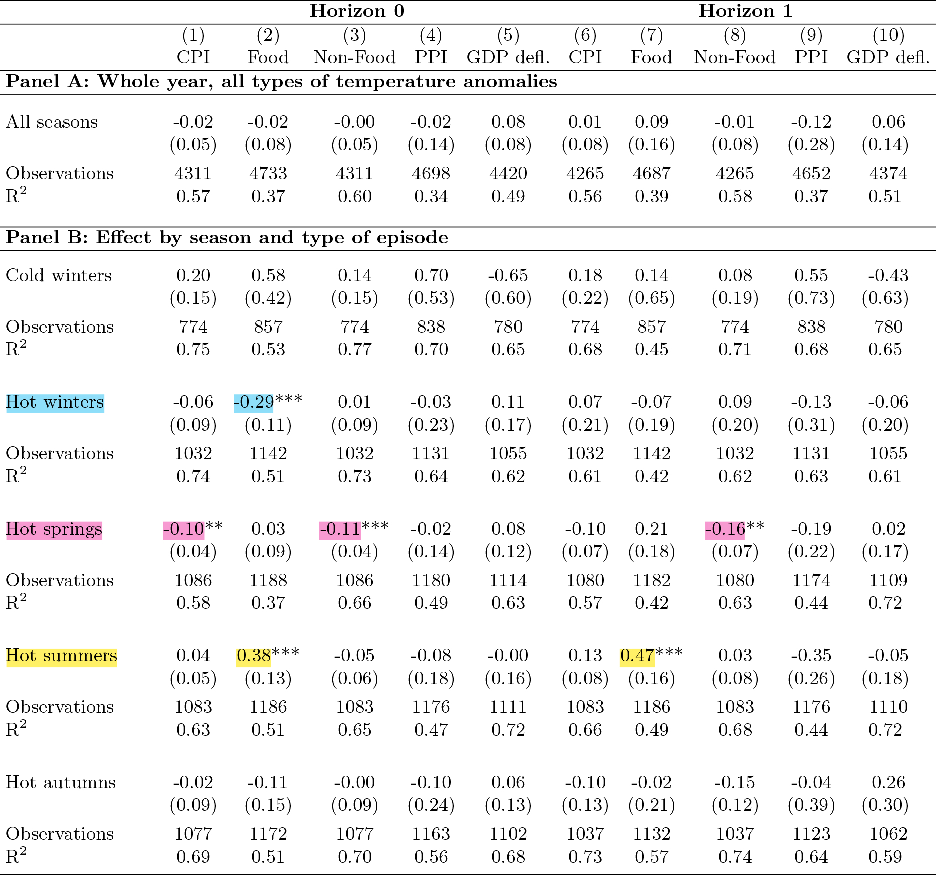
\includegraphics[width=\textwidth]{img/results_seasonss.pdf}
	\caption{}
	\source{\cite{ECB:feeling_heat}}
	\label{table:results_seasons}
\end{table}

Per ciascun coefficiente stimato $\hat{\beta}$ sono riportati: il suo valore, l'errore standard SE($\hat{\beta}$), ossia la stima della deviazione standard dello stimatore, il numero di osservazioni (anomalie) e l'indicatore sulla bontà di adattamento del modello ai dati $R^2$. Per la verifica d'ipotesi, gli autori hanno assegnato al $p$-value i seguenti livelli di significatività:

\begin{itemize}
	\item * $p<0.1$
	\item ** $p<0.05$
	\item *** $p<0.001$
\end{itemize}

Nel \textit{Panel A} si valutano gli effetti delle anomalie di temperatura sui prezzi, avendo come riferimento la temperatura media annuale di lungo periodo (1951-1980). In questo caso, per nessuno degli indici di prezzo, si ottiene un coefficiente statisticamente significativo. Ad esempio, di seguito si analizza il risultato per il \textit{Consumer Price Index} in \textit{Horizon 0}.\par

\vspace{-1em}

\begin{gather}
	\hat{\beta_1}=-0.02, SE(\hat{\beta_1})=0.05\\
	\nonumber \text{1. Sistema d'ipotesi}\\
	\nonumber \begin{cases}
		\text{H}_0:\beta_1=0 \text{ (le anomalie non producono alcun effetto sui prezzi)}\\
		\text{H}_1:\beta_1\neq0 \text{ (le anomalie hanno effetto sui prezzi)}
	\end{cases}\\
	\nonumber \text{2. Statistica }t\\
	\nonumber t=\frac{\hat{\beta_1}-0}{\text{SE}(\hat{\beta_1})} = \frac{-0.02}{0.05}=-0.4\\
	\nonumber \text{3. Valori critici con }\alpha=0.05\\
	\nonumber c=\pm1.96,\text{ quindi}\\
	\nonumber \text{si rifiuta H}_0 \text{ se }t<-1.96 \text{ oppure } t>1.96\\
	\nonumber \text{non si rifiuta H}_0 \text{ se }-1.96\le t\le 1.96\\
	\nonumber \text{4. }p \text{-value}\\
	\nonumber p\text{-value}=2\phi(-|t|)=2\phi(-0.4)=0.6892\\
	\nonumber \text{si rifiuta H}_0 \text{ se }p\text{-value} \le \alpha\\
	\nonumber \text{non si rifiuta H}_0 \text{ se }p\text{-value} > \alpha
\end{gather}

Sia la statistica $t$ $(-1.96<-0.4<1.96)$ sia il $p$-value $(0.6892>0.05)$ ci suggeriscono di non rifiutare l'ipotesi nulla H$_0$, perché il coefficiente non è statisticamente significativo. Il suo valore (-0.02) potrebbe essere frutto del caso. Ciò vale sia per i valori del trimestre corrente (\textit{Horizon 0}) sia per quelli del successivo (\textit{Horizon 1}).

Nel \textit{Panel B} il confronto avviene tra la n-esima temperatura e la media stagionale, non annuale. La variabile dummy $Temp_{c,t}$ ha un comportamento diverso rispetto a quello assunto nel \textit{Panel A}. Per ogni stagione, si studiano separatamente gli effetti degli shock positivi e di quelli negativi. I valori assunti da $Temp_{c,t}$ sono i seguenti:

\begin{table}[h]
	\centering
	\begin{tabular}{l|c|c}
		\toprule
		& $T_n < \bar{T}+1.5$°C & $T_n > \bar{T}+1.5$°C \\
		& & (shock positivo) \\
		\midrule
		$Temp_{c,t}$ & 0 & 1 \\
		\bottomrule
	\end{tabular}

	\vspace{0.5em}

	\begin{tabular}{l|c|c}
		\toprule
		& $T_n < \bar{T}-1.5$°C & $T_n > \bar{T}-1.5$°C \\
		& (shock negativo) & \\
		\midrule
		$Temp_{c,t}$ & 1 & 0 \\
		\bottomrule
	\end{tabular}
	\caption{}
	\label{tables:temp_dummy}
	\source{elaborazione propria}
\end{table}

Si~consideri ora l'indice~\textit{Food} con \textit{Horizon 0}. Nel caso di~un~inverno~nel~quale si siano verificati diversi shock di temperatura positivi,~qual~è~l'effetto sui prezzi di un inverno più caldo?

\vspace{-1.5em}

\begin{gather}
	\hat{\beta_1}=-0.29, SE(\hat{\beta_1})=0.11\\
	\nonumber \text{1. Sistema d'ipotesi}\\
	\nonumber \begin{cases}
		\text{H}_0:\beta_1=0 \text{ (le anomalie non producono alcun effetto sui prezzi)}\\
		\text{H}_1:\beta_1\neq0 \text{ (le anomalie hanno effetto sui prezzi)}
	\end{cases}\\
	\nonumber \text{2. Statistica }t\\
	\nonumber t=\frac{\hat{\beta_1}-0}{\text{SE}(\hat{\beta_1})} = \frac{-0.29}{0.11}=-2.64\\
	\nonumber \text{3. Valori critici con }\alpha=0.05\\
	\nonumber c=\pm1.96,\text{ quindi}\\
	\nonumber \text{si rifiuta H}_0 \text{ se }t<-1.96 \text{ oppure } t>1.96\\
	\nonumber \text{non si rifiuta H}_0 \text{ se }-1.96\le t\le 1.96\\
	\nonumber \text{4. }p \text{-value}\\
	\nonumber p\text{-value}=2\phi(-|t|)=2\phi(-2,64)=0.0082\\
	\nonumber \text{si rifiuta H}_0 \text{ se }p\text{-value} \le \alpha\\
	\nonumber \text{non si rifiuta H}_0 \text{ se }p\text{-value} > \alpha
\end{gather}

L'impatto di un inverno più caldo sui prezzi \textit{Food} è statisticamente significativo, così come suggerito sia dalla statistica $t$ $(-2.64 < -1.96)$ sia dal $p$-value $(0.0082~<~0.05)$. Nell'immediato il prezzo del cibo si riduce, mentre nel trimestre successivo l'effetto svanisce. Similmente, nel caso di una primavera con numerosi shock termici positivi, gli indici \textit{CPI} e \textit{Food} si riducono leggermente in \textit{Horizon 0}, mentre nel trimestre successivo l'effetto tende a scomparire. In contrasto alla tesi che si sta sostenendo, si potrebbe credere che, grazie a inverni e primavere più calde, la produzione di cibo ne gioverebbe. Ma così non è. L'effetto immediato é sì una leggera, quasi trascurabile, riduzione dei prezzi, magari dovuta a una maggiore produzione e costi energetici minori, ma questi benefici non sono persistenti e anzi, nel periodo successivo, l'estate, l'aumento di temperatura provoca effetti peggiori e più intensi.

Rilevante è l'effetto sui prezzi \textit{Food} nelle estati particolarmente calde. Mentre, nelle altre stagioni l'effetto delle anomalie sui prezzi tende a svanire, in questo caso l'impatto perdura nel tempo. I coefficienti per l'indice \textit{Food}, in entrambi gli orizzonti temporali, sono entrambi statisticamente ed economicamente significativi (Tabella~\ref{table:results_seasons}). Un'estate più calda, tipicamente caratterizzata anche da siccità, complica, rende più laboriosa e costosa la produzione di cibo. L'output della stessa si riduce e quindi genera una scarsità di risorse. Questa successione di eventi termina con il consumatore finale costretto a pagare un prezzo maggiore per il medesimo prodotto \parencite{ECB:feeling_heat}. 

L'estate sembra essere la stagione durante la quale i prezzi sarebbero più suscettibili a variazioni in caso di shock termici positivi. Per questo, gli autori hanno indagato se l'effetto sui prezzi interni dei diversi Stati sia uniforme o meno. Il campione di 48 paesi è stato diviso in due: \textit{"Advanced"} (33) e \textit{"Emerging"} (15). In Tabella \ref{table:results_splitted} vengono riportati i risultati delle regressioni prodotte dagli autori.

Per il \textit{Panel A}, il modello illustrato dall'Equazione \ref{formula:modello} viene modificato inserendo una variabile dummy che differenzia i paesi avanzati ed emergenti. I risultati non restituiscono alcun coefficiente statisticamente significativo e ciò suggerisce di indagare maggiormente.

Il \textit{Panel B} e il \textit{Panel C} si basano sulla formula dell'Equazione \ref{formula:modello}. I risultati sono emblematici: in estate, i prezzi interni dei Paesi emergenti risentono maggiormente degli shock di temperatura positivi. L'aumento colpisce sia l'indice del cibo sia quello generale, inoltre, persiste anche nel trimestre successivo. Al contrario, le economie avanzate risentono solamente di un leggero effetto positivo $(0.18)$ sui prezzi \textit{Food} del trimestre corrente (Tabella \ref{table:results_splitted}).

Entrambi i due gruppi di Paesi risentono di un effetto inflattivo sui prezzi del cibo in \textit{Horizon 0}, anche se con entità diverse. Questo aumento, molto più marcato nelle economie emergenti, si ripercuote anche sull'indice \textit{CPI} di quest'ultimi. La principale motivazione è che il cibo, nel paniere di beni costruito per questi Paesi, ricopre un peso maggiore. Ma non solo, anche la minore apertura economica verso altre economie rende queste Nazioni più dipendenti dalla produzione alimentare nazionale. Di conseguenza, avendo minori possibilità di reperire le risorse da altri paesi, uno shock dei prezzi interni viene maggiormente percepito internamente.

\begin{table}[t!]
	\centering
	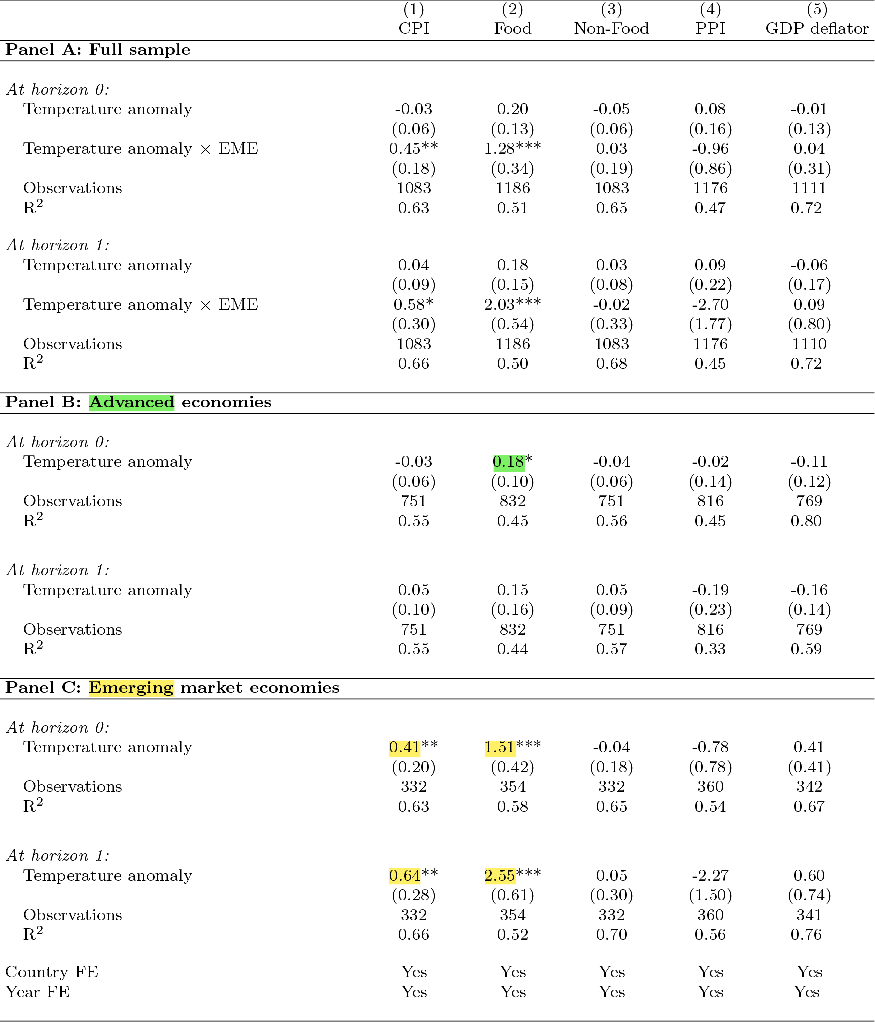
\includegraphics[width=0.95\textwidth]{img/results_seasons_countries_splitted.pdf}
	\caption{}
	\source{\cite{ECB:feeling_heat}}
	\label{table:results_splitted}
\end{table}

Questi dati ci dimostrano quanto detto in conclusione del Capitolo \ref{chp1.1}. Gli effetti del riscaldamento globale sono già visibili nella nostra vita di tutti i giorni. Periodi di siccità ed eventi climatici estremi sempre più frequenti e prolungati si stanno già verificando e stanno sprigionando le loro conseguenze, sia nei Paesi economicamente avanzati sia nei Paesi in via di sviluppo. Quest'ultimi, per di più, per la minore disponibilità di risorse, infrastrutture e, in certi casi, anche per la particolare conformazione geografica, stanno sperimentando in maniera più intensa le conseguenze di questi cambiamenti.

\begin{figure}[h]
	\centering
	\includegraphics[width=0.80\textwidth]{img/tuvalu_water.jpg}
	\caption{}
	\source{Ministry of Justice, Communication and Foreign Affairs, Tuvalu Government}
\end{figure}

Simon Kofe, ministro degli affari esteri per l'isola di Tuvalo nel Pacifico, ha tenuto il suo discorso a COP26 con l'acqua alle ginocchia \parencite{guardian:tuvalu}. Dove tutt'attorno c'è il mare, il fragile ecosistema delle Isole Pacifiche si fonda su un forte legame tra l'uomo e la terra, l'isola. Queste piccole porzioni di terra che dalle immagini satellitari si faticano a vedere, stanno sperimentando già da decenni gli effetti del cambiamento climatico: innalzamento del livello del mare, eventi atmosferici estremi e siccità prolungate.

\subsubsection{Il medio periodo}

Fino a qui, abbiamo analizzato gli effetti \textit{short term} degli shock termini positivi. Temperature maggiori hanno la capacità di infiammare, in particolare in estate, i prezzi \textit{Food}, scatenando conseguenze ambientali, economiche e sociali. Si è visto anche che, in determinati casi, gli effetti di questi eventi si possono protrarre nel tempo. Pertanto, in quest'ultima sezione, si presenteranno i risultati dello studio di Donata Faccia a riguardo degli effetti di medio periodo degli shock termici.

La Figura \ref{img:medium_term}, dividendo economie avanzate da quelle in via di sviluppo, mostra gli effetti degli shock termici positivi in estate. Partendo da \textit{Horizon~0} fino all'ottavo trimestre successivo, i grafici mostrano i valori assunti da quattro indici di prezzo, con intervalli di confidenza del 60\% e 90\%.

\begin{figure}[h]
	\centering
	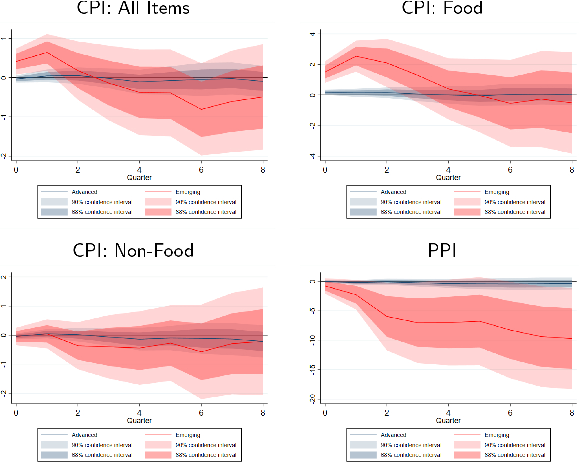
\includegraphics[width=0.8\textwidth]{img/medium_term.pdf}
	\caption{}
	\source{\cite{ECB:feeling_heat}}
	\label{img:medium_term}
\end{figure}

I Paesi avanzati risentono meno, anche nel medio periodo, degli effetti di un'estate più calda. La stima dell'andamento di tutti e quattro gli indici di prezzo mostra una capacità di questi Paesi ad adattarsi facilmente e velocemente agli shock termici. Al contrario, a seguito di un trimestre più caldo del solito, i Paesi emergenti affrontano maggiori difficoltà nel medio periodo. L'indice \textit{Food} viene interessato dallo shock per almeno i due trimestri successivi e questo si ripercuote anche sul \textit{Consumer Price Index}.

Le ampie fluttuazioni di questi indicatori, ancora una volta, evidenziano la fragilità di questi Paesi di fronte al riscaldamento globale. Di contro, le economie sviluppate non possono considerarsi al sicuro ed esenti dalle conseguenze che il cambiamento climatico sta già producendo e che continuerà a fare. Loro compito è, grazie alle maggiori risorse a loro disposizione, avviare un progresso tecnologico che permetta di diminuire la nostra impronta climatica, ossia riducendo la produzione di gas clima alteranti, presentati nel Capitolo \ref{chp1.1}.

\subsection{Ultime considerazioni}

In conclusione e a sostegno dell'importanza dei temi trattati in queste pagine, si propongono due ultime considerazioni.

L'inflazione deve essere gestita dalle Banche centrali. Sulla carta, perché questo compito, nel caso della BCE, rappresenta il suo primo mandato a cui è chiamata ad assolvere. Nella pratica, perché il governo dei prezzi tutela il potere di acquisto delle persone, in particolare di quelle fasce di popolazione con salari al di sotto della media e che quindi risentono maggiormente del costo inflazionistico. Il controllo dell'inflazione non è più solamente una supervisione dei cicli economici e monetari, ma anche uno strumento di tutela sociale.

Il cambiamento climatico e il riscaldamento globale sono realtà, così come i loro effetti. I dati dello studio preso in esame hanno dimostrato che questi due eventi sono in grado di alterare la dinamica dei prezzi. Più in generale, le loro conseguenze modificano il modo in cui siamo abituati a vivere oggi. Qualche anno fa, Papa Francesco esordì dicendo: \textit{"Vivere sani in un mondo malato è utopia"}. L'inquinamento e il cambiamento climatico possono influire negativamente anche sulla salute delle persone. La Dichiarazione Universale dei Diritti Umani non prevede esplicitamente un diritto dell'uomo ad un ambiente pulito e sicuro e per questo, in questi anni, le organizzazioni internazionali si sono mobilitate per riconoscere tutele e nuovi principi \parencite{hrc:europe}. Il risultato di questo dialogo è stata la Risoluzione A/HRC/RES/48/13 del Consiglio sui Diritti Umani delle Nazioni Unite raggiunta l'8 ottobre 2021 \parencite{hrc:risoluzione}. Il primo e più importante punto di questo documento è il riconoscimento del diritto, umano e universale, a un ambiente pulito, salutare e sostenibile, quale elemento necessario per il godimento di tutti gli altri diritti umani.

Non si nasce liberi e uguali se l'ambiente in cui si cresce è ostile. Non si vive in salute se l'ambiente che si abita è inquinato. E non si può avere liberamente accesso al cibo se quest'ultimo è troppo costoso.

\backmatter
\chapter{Conclusioni}

L'esposizione fin qui svolta ci permette di giungere ad alcune conclusioni.

L'attività umana è responsabile del cambiamento climatico in atto. Con riguardo non solo agli effetti diretti, per esempio la crescente concentrazione in atmosfera di sostanze inquinanti, ma anche degli effetti indiretti dovuti al riscaldamento globale, come le siccità prolungate, gli eventi atmosferici estremi e l'acidificazione delle acque marine. Queste conseguenze stanno interferendo con il nostro normale modo di vivere, ad esempio riducendo la disponibilità di acqua per l'agricoltura o innalzando il livello del mare.

L'inflazione, oggi, è fuori controllo. Le Banche centrali non sono state in grado di mantenerla entro i propri target. Questo fenomeno è il risultato di una combinazione di diversi fattori, in parte non sotto il loro diretto controllo: le tensioni geopolitiche ed energetiche, la ripresa dell'economia globale post pandemia e l'enorme disponibilità di moneta nei mercati. Nei mesi futuri, la politica monetaria dovrà impegnarsi a riportare i prezzi sotto controllo, tenendo presente che questo obiettivo è dovuto innanzitutto nei confronti del potere di acquisto delle persone.

Si potrebbe credere che questi due fenomeni viaggino su due binari paralleli, ma, come si è visto, in realtà interferiscono tra loro. Il riscaldamento globale influenza i prezzi \textit{Food}, sia nei Paesi avanzati sia in quelli emergenti. L'impatto sui prezzi di quest'ultimi Paesi però, è più elevato e prolungato nel tempo. Il \textit{working paper} di Donata Faccia ha inoltre permesso di evidenziare che gli effetti dell'aumento di temperatura differiscono dal momento in cui questi si verificano: l'estate è il periodo in cui i prezzi aumentano in modo statisticamente ed economicamente significativo, mentre, in inverno e primavera, questi diminuiscono leggermente.

Così come è stata definita da Isabel Schnabel, la \textit{climateflation}, ossia i nuovi costi legati al cambiamento climatico, è realtà.

Entrambi i temi fin qui trattati non possono più essere ignorati o affrontati solo ideologicamente. Per essere risolti, o almeno mitigati, necessitano di azioni complesse, di lungo periodo, ma concrete. Le poste in gioco sono, prima, gli equilibri sociali così come li conosciamo noi oggi e, poi, la vivibilità del pianeta Terra.

